\subsection{Optimization Aggressiveness with Osmotic Scaling}
We already learned from the experiment about load balancer scale that there is a tendency for a higher scale of load balancers to ultimately result in better performance.
With this experiment we want to test the interplay of this phenomenon with the osmotic load balancing and scaling we propose. With our osmotic approach we can set the scale-up threshold to more or less arbitrary values to influence how quickly or slowly the system scales up the number of load balancers, and how many load balancers will thus ultimately end up being deployed.

\subsubsection{Setup}
To test the performance we simulate a number of different configuration scenarios. For the rest of the system environment we choose to reuse the globally distributed topology from previous experiments with a request rate of 75\gls{rps} being simulated over the course of 2000 seconds.

For the parameters of the osmotic scaling and scheduling we run experiments for a range of scale-up thresholds ranging from 0.02 to 0.1.
The scale down threshold is always set to 0.2, which is relatively high, because we explicitly want to test how the scale-up threshold can be used to determine how many load balancers the system will deploy to optimize response times.

\subsubsection{Results}

\begin{table}[]
\begin{tabular}{lrrrrr}
\hline
\textbf{\begin{tabular}[c]{@{}l@{}}Upscaling\\ Pressure\\ Threshold\end{tabular}} & \textbf{\begin{tabular}[c]{@{}r@{}}LB\\ Replicas\end{tabular}} & \textbf{\begin{tabular}[c]{@{}r@{}}Mean\\ TRT\end{tabular}} & \textbf{\begin{tabular}[c]{@{}r@{}}Mean\\ FET\end{tabular}} & \textbf{\begin{tabular}[c]{@{}r@{}}Mean\\ LB\_FX\end{tabular}} & \textbf{\begin{tabular}[c]{@{}r@{}}Mean\\ CL\_LB\end{tabular}} \\ \hline
0.1                                                                               & 4                                                              & 155.8ms                                                     & 29.1ms                                                      & 33.5ms                                                         & 92.7ms                                                         \\
0.09                                                                              & 4                                                              & 152.5ms                                                     & 29.7ms                                                      & 30.1ms                                                         & 92.2ms                                                         \\
0.08                                                                              & 6                                                              & 152.1ms                                                     & 29.5ms                                                      & 30.0ms                                                         & 92.2ms                                                         \\
0.07                                                                              & 5                                                              & 152.5ms                                                     & 29.3ms                                                      & 30.4ms                                                         & 92.4ms                                                         \\
0.06                                                                              & 5                                                              & 148.5ms                                                     & 29.6ms                                                      & 26.6ms                                                         & 91.6ms                                                         \\
0.05                                                                              & 5                                                              & 147.5ms                                                     & 29.9ms                                                      & 25.3ms                                                         & 91.3ms                                                         \\
0.04                                                                              & 5                                                              & 148.5ms                                                     & 29.8ms                                                      & 26.5ms                                                         & 91.5ms                                                         \\
0.03                                                                              & 7                                                              & 136.8ms                                                     & 26.4ms                                                      & 19.6ms                                                         & 91.2ms                                                         \\
0.02                                                                              & 20                                                             & 139.0ms                                                     & 24.8ms                                                      & 25.3ms                                                         & 90.2ms                                                         \\ \hline
\end{tabular}
\caption{Response time performance metrics for different upscaling pressure thresholds}
\label{tab:osmotic_scaling_aggressiveness}
\end{table}





\begin{figure}
    \centering
    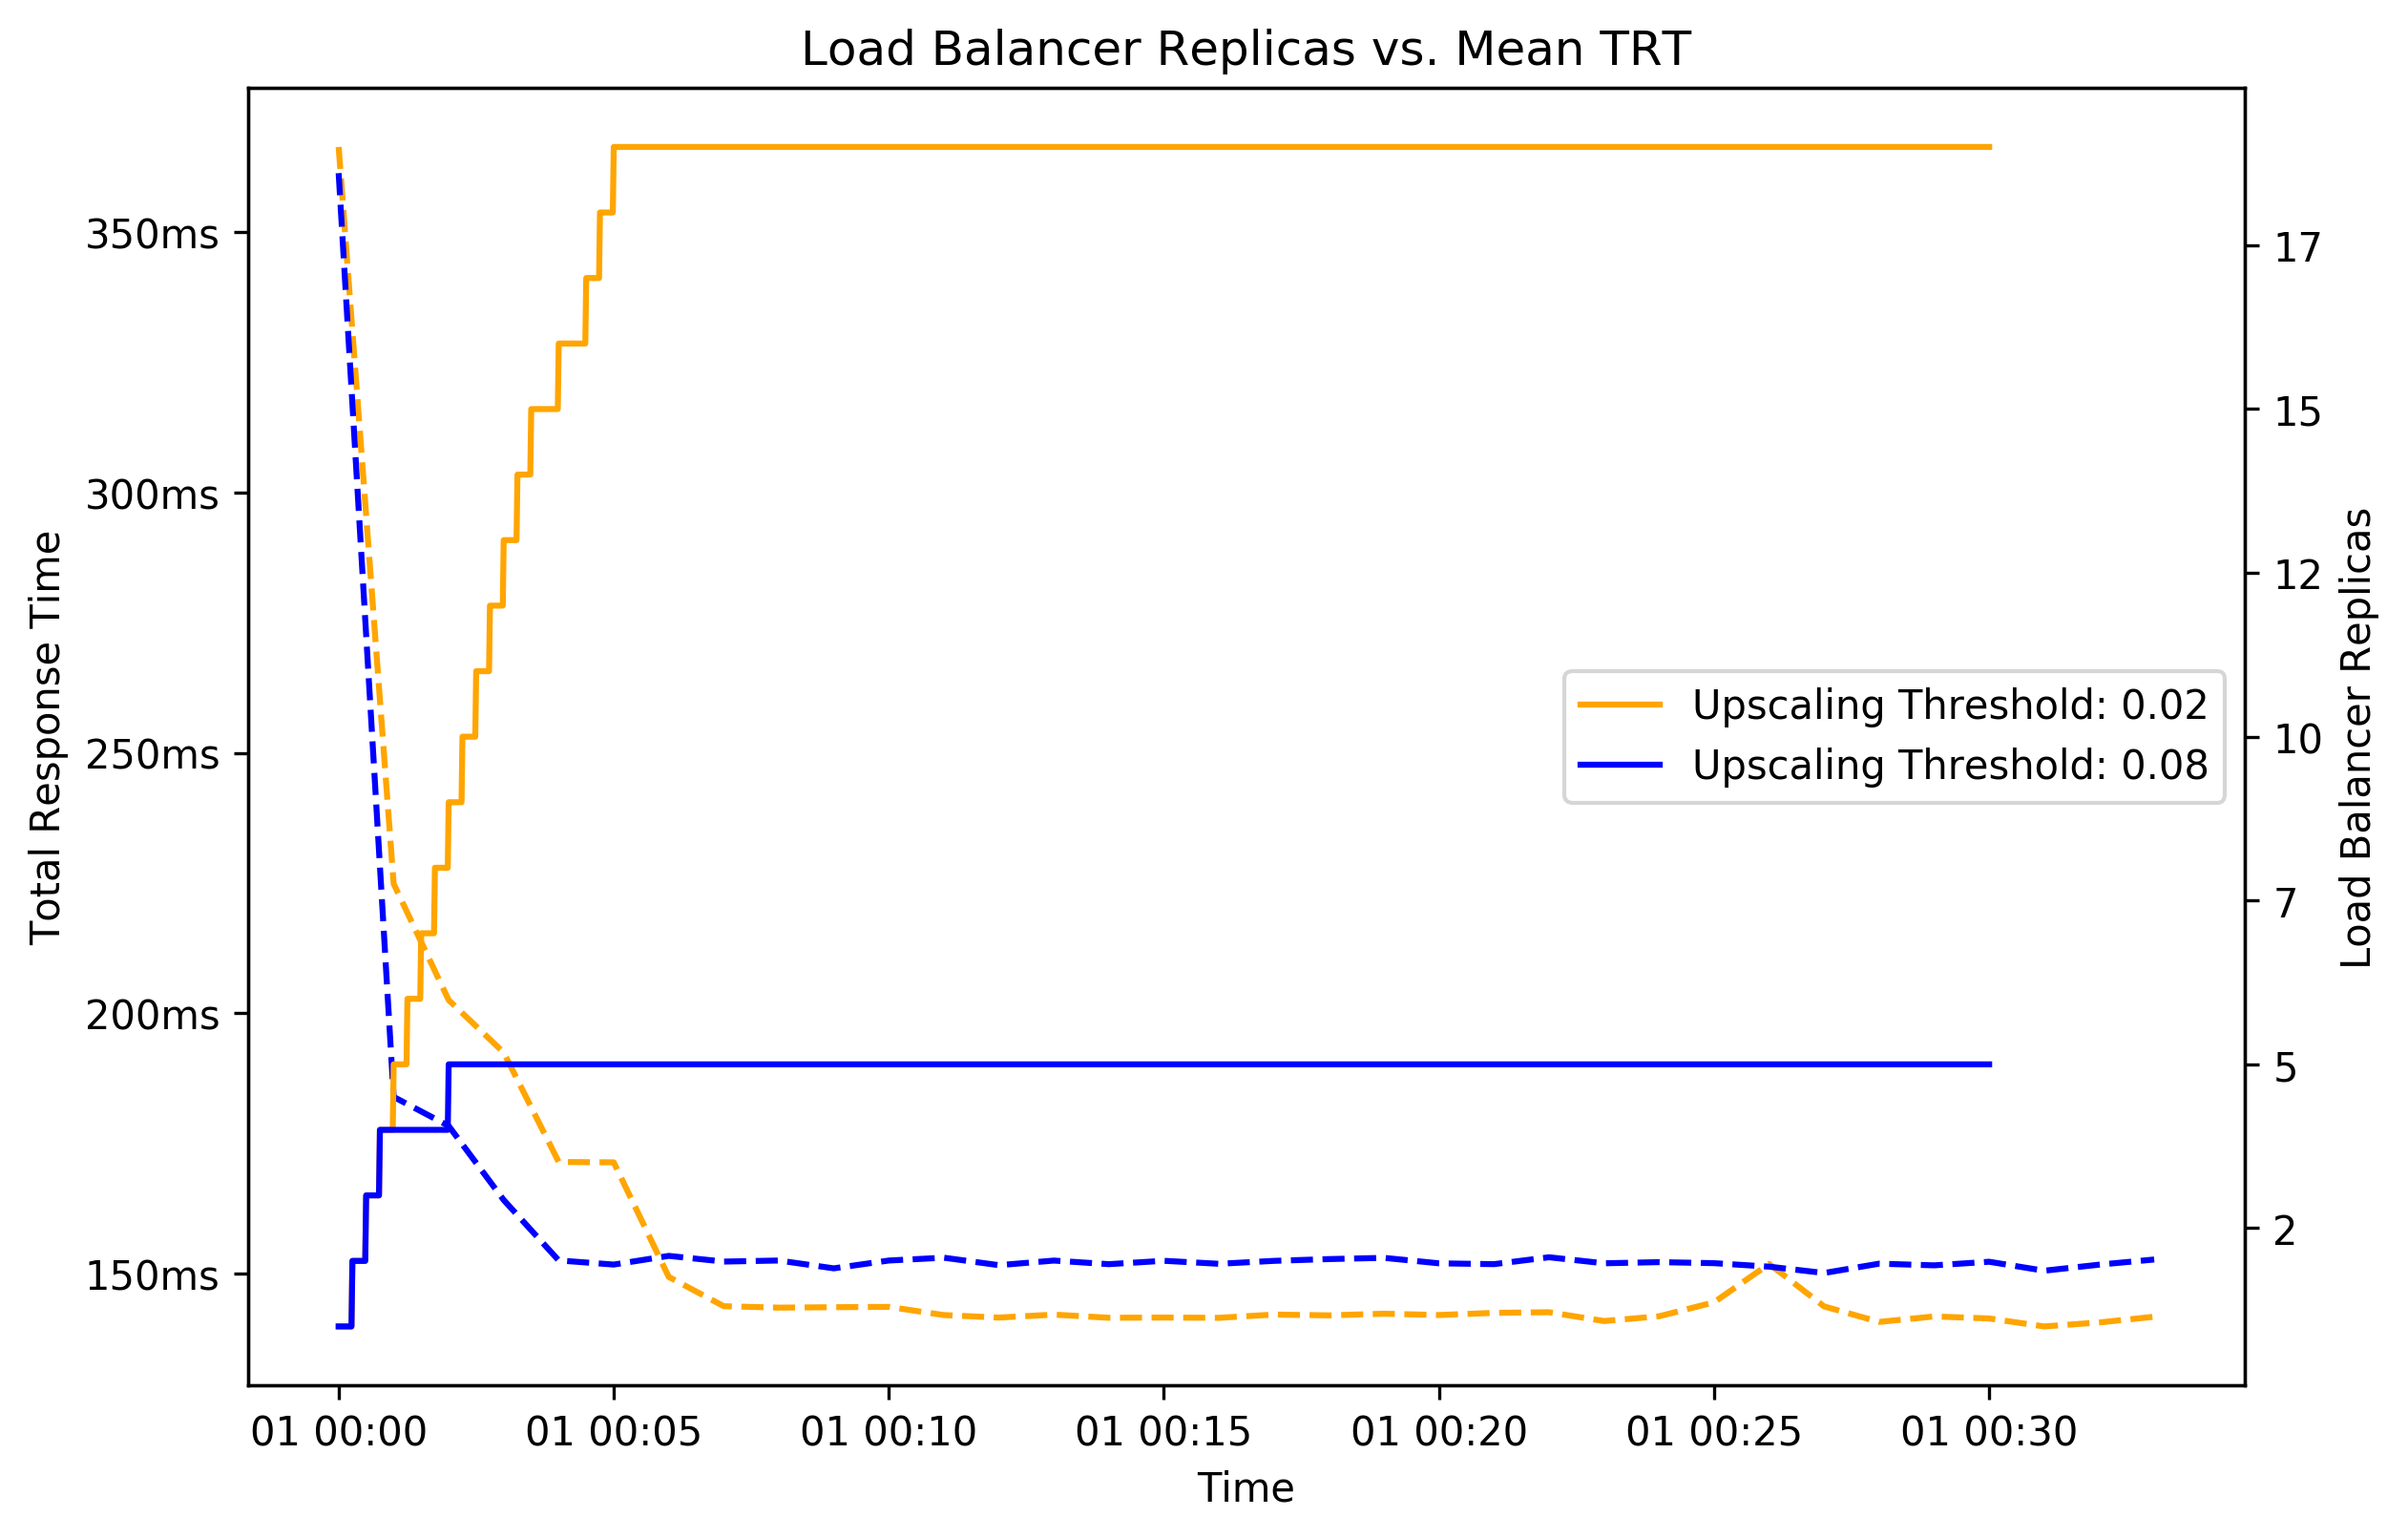
\includegraphics[width=12cm]{graphics/graphs/osmotic_optim_thres_vs_trt.png}
    \caption{\gls{trt} compared to current load balancer scale for two different osmotic scaling parametrizations}
    \label{fig:osmotic_trt_vs_replica_scale}
\end{figure}

The results show two clear trends.
First that will lower upscaling pressure thresholds more load balancer replicas are being deployed by the osmotic scaling component, and second that the mean response time improves with higher number of load balancer replicas.
As Table \ref{tab:osmotic_scaling_aggressiveness} shows, there is a diminishing return with higher numbers of load balancers, at least in the topology scenario tested.
The results also show that while higher numbers of load balancers provide better performance once the load balancers have gathered enough information about available replicas, this process is faster the fewer load balancers there are, thus giving better performance early on.
The behaviour can be observed easily in the graph in Figure \ref{fig:osmotic_trt_vs_replica_scale}.